% !TEX TS-program = pdflatex
% Overleaf: blank project; compiler = pdfLaTeX; no extra files.
\documentclass[aspectratio=169]{beamer}
\usetheme{Madrid}
\usecolortheme{default}
\usepackage{booktabs,array}
\usepackage{pgfplots}
\pgfplotsset{compat=1.17}
\setbeamertemplate{navigation symbols}{}
\setbeamertemplate{footline}[frame number]

\title{Tricycle on Cerium: Nonlinear Layers and Bootstrapping}
\subtitle{Results as of November 23}
\author{Sagnik Biswas}
\date{November 23, 2026}

\begin{document}

\begin{frame}
  \titlepage
\end{frame}

\begin{frame}{Summary}
\small
\begin{enumerate}\small
  \item \textbf{Counted Tricycle's bootstraps} from its source: 16--24 per layer, 222 for BERT-Base.
  \item \textbf{Measured Cerium's bootstrap} on the H100: 21.3 ms, adds $3.3\times10^{-6}$ error.
  \item \textbf{Ran Tricycle's GELU, LayerNorm and softmax encrypted on Cerium}, with Tricycle's algorithms and degree-119 polynomials. All accurate.
  \item \textbf{Put the bootstrap inside the program} for LayerNorm and softmax, using Cerium BERT's own bootstrap.
\end{enumerate}
\vspace{0.6em}
\begin{block}{Headline}
Summing the separately measured parts, one Tricycle layer on Cerium is about 1.0 s of GPU time, against 3.4 s for Cerium's own BERT-Base layer. Not yet a single fused layer.
\end{block}
\end{frame}

\begin{frame}{How many bootstraps Tricycle needs}
\small
Read from Tricycle's SST-2 code (128 tokens). Most bootstraps pack two real ciphertexts into one complex one.
\begin{center}\footnotesize
\begin{tabular}{@{}llll@{}}
\toprule
\textbf{Layers} & \textbf{Softmax normalization} & \textbf{Wide GELU features} & \textbf{Bootstraps per layer}\\
\midrule
1, 2, 12 & direct reciprocal & no & 16\\
3 & reciprocal, then two inverse square roots & no & 20\\
4--9 & two inverse square roots & no & 18\\
10 & direct reciprocal & yes & 22\\
11 & two inverse square roots & yes & 24\\
\bottomrule
\end{tabular}
\end{center}
\begin{itemize}\small
  \item 222 for 12 layers, 18.5 per layer on average.
  \item Cerium's 32K-slot bootstrap on the H100: \textbf{21.3 ms} wall, 22.3 ms kernel time, output at 19 limbs (9 levels), error $3.3\times10^{-6}$.
\end{itemize}
\end{frame}

\begin{frame}{Tricycle's nonlinear kernels on Cerium, run separately}
\small
\begin{center}\footnotesize
\begin{tabular}{@{}lrrll@{}}
\toprule
\textbf{Kernel (BERT-Base shapes)} & \textbf{Wall time} & \textbf{Kernel time} & \textbf{CKKS error} & \textbf{vs exact function}\\
\midrule
GELU, 16 blocks & 111.4 ms & 144.2 ms & $1.7\times10^{-8}$ & $5.6\times10^{-5}$\\
LayerNorm, 4 blocks & 39.4 ms & 69.9 ms & $3.7\times10^{-9}$ & $3.7\times10^{-9}$\\
Softmax, 4 $\times$ 4 score blocks & 68.5 ms & 114.8 ms & $1.9\times10^{-8}$ & $1.2\times10^{-2}$\\
\bottomrule
\end{tabular}
\end{center}
\begin{itemize}\small
  \item Bootstraps not included: post-bootstrap values enter as fresh ciphertexts.
  \item Softmax's $1.2\times10^{-2}$ is Tricycle's own $(1+x/256)^{256}$ exponential, not encryption error.
  \item \textbf{Rotation noise:} each rotation adds about $2^{52}$. Rotated values are kept one prime higher ($2^{83}$) at no level cost. Without that, LayerNorm was off by 0.08.
  \item \textbf{Fewer levels:} Cerium's bootstrap gives 9 levels where Tricycle plans for HEaaN's 12. Two exact rewrites close the gap.
\end{itemize}
\end{frame}

\begin{frame}{New: bootstrapping inside the program}
\small
Pre-bootstrap work, then Cerium BERT's real bootstrap, then the rest, in \textbf{one encrypted program}:
\begin{center}\footnotesize
\begin{tabular}{@{}lrrll@{}}
\toprule
\textbf{Fused kernel} & \textbf{Bootstraps} & \textbf{Wall time} & \textbf{CKKS error} & \textbf{vs exact function}\\
\midrule
LayerNorm, 4 blocks & 1 & 63.6 ms & $1.3\times10^{-5}$ & $1.3\times10^{-5}$\\
Softmax, 4 $\times$ 4 score blocks & 20 & 543 ms & $1.6\times10^{-4}$ & $1.2\times10^{-2}$\\
\bottomrule
\end{tabular}
\end{center}
\begin{itemize}\small
  \item Matches the separate measurements: LayerNorm 39.4 + 21.3 $\approx$ 61 ms; softmax 68.5 + 20 $\times$ 21.3 $\approx$ 495 ms.
  \item Softmax is as accurate as Tricycle's exponential allows (same $1.2\times10^{-2}$ as before).
  \item Softmax bootstraps 20 ciphertexts one by one. Tricycle packs them into 6, using a free multiply-by-$i$ that Cerium lacks. Packing two per bootstrap would roughly halve this.
\end{itemize}
\end{frame}

\begin{frame}{Getting the bootstrap accurate: input headroom}
\small
\begin{columns}[T]
\begin{column}{0.52\textwidth}
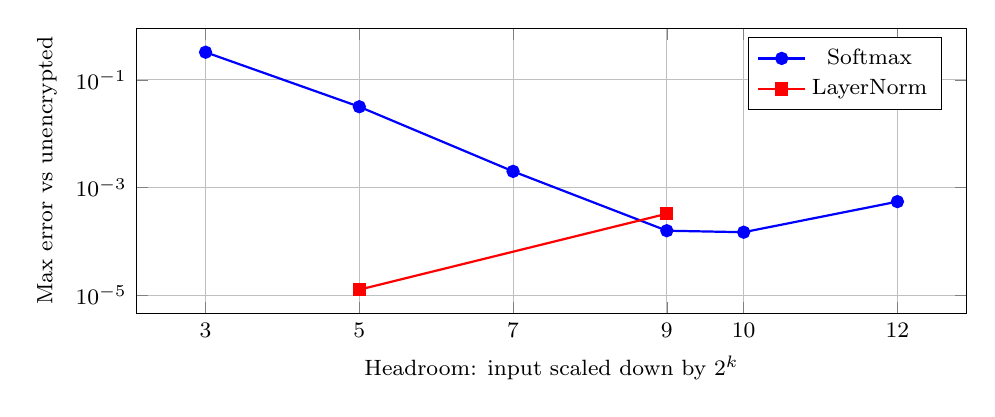
\begin{tikzpicture}
\begin{semilogyaxis}[
  width=\linewidth, height=5.2cm,
  xlabel={Headroom: input scaled down by $2^{k}$},
  ylabel={Max error vs unencrypted},
  xtick={3,5,7,9,10,12},
  legend pos=north east, legend style={font=\footnotesize},
  tick label style={font=\footnotesize}, label style={font=\footnotesize},
  grid=major]
\addplot[mark=*, blue, thick] coordinates {(3,0.3245) (5,0.03162) (7,0.002001) (9,0.0001586) (10,0.0001488) (12,0.0005491)};
\addlegendentry{Softmax}
\addplot[mark=square*, red, thick] coordinates {(5,0.00001279) (9,0.0003274)};
\addlegendentry{LayerNorm}
\end{semilogyaxis}
\end{tikzpicture}
\end{column}
\begin{column}{0.46\textwidth}
\begin{itemize}\small
  \item Each value is scaled down by $2^{k}$ before the bootstrap and back up after. Cerium's BERT uses up to $2^{14}$.
  \item Too little headroom: the input leaves the bootstrap's valid range (0.32 at $2^3$).
  \item Too much: the bootstrap's fixed noise gets relatively larger.
  \item Best: $2^5$ for LayerNorm, $2^9$--$2^{10}$ for softmax.
  \item Bootstrapping the exponential later (after 5 of 8 squarings instead of 3) did not help.
\end{itemize}
\end{column}
\end{columns}
\end{frame}

\begin{frame}{One layer, summed from separate measurements}
\small
Layers 1, 2 and 12 (direct softmax, 16 bootstraps), GPU kernel time per layer:
\begin{center}\footnotesize
\begin{tabular}{@{}lrr@{}}
\toprule
\textbf{Part} & \textbf{Cerium BERT-Base} & \textbf{Tricycle on Cerium}\\
\midrule
Matrix multiplications & 1{,}125 ms & 245 ms\\
Bootstrapping & 1{,}747 ms & 357 ms (16 $\times$ 22.3 ms)\\
GELU & 276 ms & 144 ms\\
Softmax & 234 ms & 115 ms\\
LayerNorm (two) & 15 ms & 140 ms\\
\midrule
\textbf{Total} & \textbf{3{,}403 ms} & \textbf{about 1{,}000 ms}\\
\bottomrule
\end{tabular}
\end{center}
{\footnotesize Caveats: assumes Tricycle's packed bootstraps (16), which need the multiply-by-$i$ packing not yet built on Cerium; the fused softmax alone currently uses 20. One level gap between softmax and $PV$ is unresolved. Matmuls were timed at lower input levels than a fused layer needs. LayerNorm is Tricycle's slowest part here: four degree-119 polynomials and 182 rotations.}
\end{frame}

\begin{frame}{Next steps}
\small
\begin{block}{Done}
\begin{itemize}\small
  \item All three nonlinear kernels accurate on Cerium. LayerNorm and softmax run with the real bootstrap inside.
\end{itemize}
\end{block}
\begin{block}{Next}
\begin{itemize}\small
  \item Pack two real ciphertexts per bootstrap for softmax (20 $\to$ about 10).
  \item Fuse GELU's bootstrap and the feed-forward matmuls; close the softmax-to-$PV$ level gap.
  \item Inverse-square-root softmax for layers 3--9 and 11.
  \item One complete encrypted layer, timed end to end against Cerium's 3.4 s.
\end{itemize}
\end{block}
\end{frame}

\end{document}
